\section{Aplicacao empirica: regimes inflacionarios do IPCA}

Esta secao aplica cadeias de Markov em tempo discreto a dinamica da inflacao brasileira. A variavel observada e o IPCA mensal, obtido da serie 433 do Sistema Gerenciador de Series Temporais do Banco Central do Brasil. A amostra utilizada vai de janeiro de 1980 a abril de 2026, totalizando 556 observacoes mensais. O objetivo empirico e avaliar se os regimes inflacionarios apresentam dependencia temporal, qual a persistencia esperada de cada regime e se a matriz de transicao permaneceu estavel antes e depois do Plano Real.

A estrategia empirica e deliberadamente discreta. Em vez de modelar diretamente o valor continuo do IPCA, cada observacao mensal e classificada em um dos tres estados:
\[
S=\{\text{Baixa},\text{Moderada},\text{Alta}\}.
\]
Essa transformacao permite estimar uma cadeia de Markov finita e interpretar a inflacao brasileira em termos de probabilidades de permanencia e transicao entre regimes.

Para evitar uma desconexao entre o referencial teorico e a aplicacao empirica, a Tabela \ref{tab:ponte_teoria_aplicacao} explicita quais conceitos sao operacionalizados nos dados e quais permanecem apenas como enquadramento teorico. O nucleo empirico do trabalho e uma cadeia de Markov finita, homogenea no tempo, estimada em frequencia mensal. Portanto, conceitos como distribuicao estacionaria, classificacao dos estados, periodicidade, autovalores, gap espectral, inferencia por verossimilhanca e testes de dependencia temporal sao diretamente usados na aplicacao. Por outro lado, tempo continuo, acoplamento e dependencia fraca sao mantidos como extensoes conceituais: ajudam a situar o tema em probabilidade aplicada, mas nao sao estimados diretamente com os dados do IPCA.

\begin{table}[H]
\centering
\caption{Relacao entre conceitos teoricos e uso na aplicacao empirica}
\label{tab:ponte_teoria_aplicacao}
\begin{tabular}{p{0.34\textwidth}p{0.56\textwidth}}
\hline
Conceito teorico & Uso na aplicacao ao IPCA \\
\hline
Matriz de transicao e verossimilhanca & Estimacao de \(\widehat{P}\) por contagens de transicoes mensais entre regimes. \\
Classificacao dos estados & Verificacao de comunicacao entre estados, irreducibilidade e aperiodicidade da matriz empirica. \\
Distribuicao estacionaria & Calculo de \(\pi\) como resumo probabilistico da matriz agregada, com interpretacao cautelosa devido ao Plano Real. \\
Teoria espectral e mistura & Calculo de autovalores, gap espectral e limite superior aproximado para tempo de mistura. \\
Inferencia para cadeias finitas & Intervalos bootstrap, testes LR e p-valores de Monte Carlo. \\
Acoplamento & Nao estimado empiricamente; usado apenas como motivacao teorica para convergencia/mistura. \\
Tempo continuo & Nao estimado, pois o IPCA e mensal; permanece como extensao teorica fora do escopo empirico. \\
Dependencia fraca & Nao testada formalmente; a aplicacao testa dependencia temporal discreta entre regimes. \\
\hline
\end{tabular}
\end{table}

\subsection{Classificacao dos regimes}

Como a amostra cobre tanto a fase de inflacao cronica dos anos 1980 e inicio dos anos 1990 quanto o periodo de estabilizacao posterior ao Plano Real, limites fixos como 0,3\% ou 0,7\% ao mes seriam inadequados para a amostra completa. Por isso, a classificacao principal usa tercis da distribuicao historica do IPCA. O primeiro tercil define a fronteira entre inflacao baixa e moderada, enquanto o segundo tercil define a fronteira entre inflacao moderada e alta.

\begin{table}[H]
\centering
\caption{Limiares dos regimes inflacionarios na amostra completa}
\label{tab:limiares_globais}
\begin{tabular}{lc}
\hline
Limite & IPCA mensal (\%) \\
\hline
Baixa--Moderada & 0,46 \\
Moderada--Alta & 1,61 \\
\hline
\end{tabular}
\end{table}

Assim, meses com IPCA inferior a 0,46\% sao classificados como regime de baixa inflacao; meses entre 0,46\% e 1,61\% sao classificados como regime moderado; e meses acima de 1,61\% sao classificados como regime de alta inflacao. Por construcao, os tres regimes ficam aproximadamente balanceados na amostra completa: 185 meses em baixa inflacao, 186 em inflacao moderada e 185 em inflacao alta.

\begin{figure}[H]
\centering
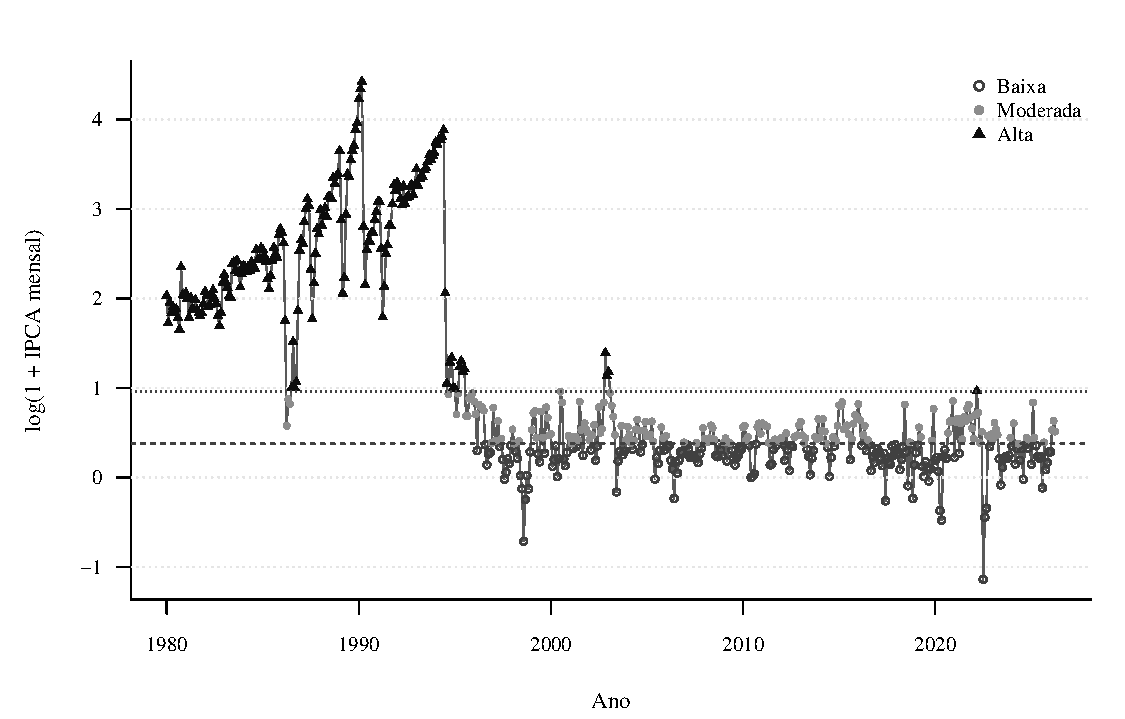
\includegraphics[width=0.85\textwidth]{resultados_markov_ipca/grafico_09_ipca_log1p_regimes.pdf}
\caption{IPCA mensal em escala logaritmica e classificacao em regimes.}
\label{fig:ipca_log_regimes}
\end{figure}

A Figura \ref{fig:ipca_log_regimes} apresenta o IPCA em escala \(\log(1+\text{IPCA})\). A escala logaritmica e usada apenas para visualizacao, pois a amostra desde 1980 contem valores muito elevados de inflacao mensal no periodo anterior ao Plano Real. O grafico evidencia que a dinamica inflacionaria brasileira nao e homogenea ao longo do tempo: a fase pre-Real concentra os episodios de maior inflacao, enquanto o periodo posterior a julho de 1994 apresenta niveis muito menores e mais estaveis.

\subsection{Matriz de transicao, persistencia e diagnosticos formais}

Depois de classificar cada mes em um dos tres regimes, estima-se a matriz de transicao por maxima verossimilhanca. Seja \(n_{ij}\) o numero de transicoes observadas do estado \(i\) para o estado \(j\). A estimativa e dada por
\[
\widehat{p}_{ij}=\frac{n_{ij}}{\sum_j n_{ij}}.
\]

\begin{table}[H]
\centering
\caption{Matriz de transicao estimada para os regimes do IPCA, com contagens entre parenteses}
\label{tab:matriz_transicao_contagens}
\begin{tabular}{lccc}
\hline
Origem \(\backslash\) Destino & Baixa & Moderada & Alta \\
\hline
Baixa    & 0,7027 (130) & 0,2973 (55)  & 0,0000 (0) \\
Moderada & 0,2973 (55)  & 0,6757 (125) & 0,0270 (5) \\
Alta     & 0,0000 (0)   & 0,0324 (6)   & 0,9676 (179) \\
\hline
\end{tabular}
\end{table}

A Tabela \ref{tab:matriz_transicao_contagens} mostra que a matriz possui elevada persistencia na diagonal principal, especialmente no regime de alta inflacao. Condicionalmente a economia estar em regime alto, a probabilidade estimada de permanecer em alta no mes seguinte e 0,9676. As transicoes diretas Baixa \(\rightarrow\) Alta e Alta \(\rightarrow\) Baixa aparecem com probabilidade estimada igual a zero porque nao foram observadas na amostra. Essa leitura e amostral, nao estrutural: zero observado nao implica impossibilidade economica.

\begin{table}[H]
\centering
\caption{Persistencia e duracao esperada dos regimes na amostra completa}
\label{tab:persistencia_global}
\begin{tabular}{lcc}
\hline
Regime & Probabilidade de permanencia & Duracao esperada (meses) \\
\hline
Baixa    & 0,7027 & 3,36 \\
Moderada & 0,6757 & 3,08 \\
Alta     & 0,9676 & 30,83 \\
\hline
\end{tabular}
\end{table}

A duracao esperada de cada regime e calculada por \(E(D_i)=1/(1-\widehat{p}_{ii})\), desde que \(\widehat{p}_{ii}<1\). Na amostra completa, a duracao esperada do regime de alta inflacao e 30,83 meses. Esse valor deve ser interpretado com cautela, pois a amostra completa combina dois ambientes monetarios muito distintos. A persistencia agregada da alta inflacao e fortemente influenciada pela sequencia de meses de inflacao cronica antes da estabilizacao.

A distribuicao estacionaria estimada e
\[
\pi=(0,3529;\,0,3529;\,0,2941),
\]
respectivamente para os regimes Baixa, Moderada e Alta. O uso de ponto e virgula evita ambiguidade com a convencao brasileira de virgula decimal. Essa distribuicao representa a proporcao de tempo que a cadeia tenderia a passar em cada regime caso a matriz estimada permanecesse constante indefinidamente. Como houve mudanca institucional relevante com o Plano Real, essa distribuicao deve ser lida como resumo probabilistico da matriz agregada, e nao como previsao estrutural de longo prazo.

Para conectar a aplicacao empirica aos conceitos teoricos discutidos anteriormente, foram calculados diagnosticos formais da matriz estimada. A cadeia empirica e irredutivel porque todos os estados se comunicam por algum numero finito de passos: embora nao haja transicoes diretas observadas entre Baixa e Alta, ambas se conectam por meio do estado Moderada. A cadeia tambem e aperiodica, pois cada estado possui probabilidade positiva de permanencia, isto e, \(\widehat{p}_{ii}>0\).

A reversibilidade foi avaliada pela condicao de balanco detalhado,
\[
\pi_i p_{ij}=\pi_j p_{ji}, \quad \forall i,j.
\]
Na matriz estimada, o maior desvio absoluto de balanco detalhado foi
\[
\max_{i,j}|\pi_i p_{ij}-\pi_j p_{ji}|=1,39\times 10^{-17}.
\]
Como esse residuo e inferior ao criterio numerico de \(10^{-8}\), a matriz foi classificada como aproximadamente reversivel. Essa conclusao e numerica, nao teorica: ela decorre da matriz empirica estimada.

Para a analise espectral, os autovalores da matriz foram ordenados por modulo. O segundo maior autovalor em modulo e \(|\lambda_2|=0,9552\), produzindo gap espectral
\[
\gamma=1-|\lambda_2|=0,0448.
\]
O tempo de mistura reportado nao e um calculo exato da distancia de variacao total. Trata-se de um limite superior espectral aproximado, usado para fins diagnosticos:
\[
t_{\text{mix}}(\varepsilon)
\leq
\left\lceil
\frac{\log\left[1/(\varepsilon\sqrt{\pi_{\min}})\right]}{\gamma}
\right\rceil,
\]
em que \(\pi_{\min}=0,2941\), \(\gamma=0,0448\) e \(\varepsilon=0,05\). Substituindo esses valores, obtem-se \(t_{\text{mix}}(0,05)\leq 81\) meses. Portanto, o numero deve ser interpretado como indicacao de convergencia lenta, e nao como tempo exato de mistura.

\begin{table}[H]
\centering
\caption{Diagnosticos formais da matriz de transicao empirica}
\label{tab:diagnosticos_markov}
\begin{tabular}{lc}
\hline
Diagnostico & Resultado \\
\hline
Irredutivel & Sim \\
Aperiodica & Sim \\
Reversivel aproximadamente & Sim \\
Segundo maior autovalor em modulo & 0,9552 \\
Gap espectral & 0,0448 \\
Limite superior espectral para \(t_{\text{mix}}(0,05)\) & 81 meses \\
\hline
\end{tabular}
\end{table}

O pequeno gap espectral indica convergencia lenta para a distribuicao estacionaria, coerente com a elevada persistencia do regime de alta inflacao. Esse resultado operacionaliza a nocao teorica de mistura no caso empirico do IPCA, mas deve ser lido como diagnostico aproximado.

\subsection{Inferencia estatistica}

A matriz de transicao e uma estimativa pontual. Para avaliar a incerteza amostral, foram usados intervalos de confianca assintoticos, bootstrap parametrico e testes de razao de verossimilhanca. Como ha zeros amostrais na matriz de contagens, o bootstrap foi conduzido a partir de uma matriz suavizada com \(\alpha=0,5\). A matriz suavizada e usada apenas para simular trajetorias artificiais; a estimativa pontual reportada permanece sendo a estimativa de maxima verossimilhanca. Foram usadas \(B=1000\) replicacoes bootstrap.

\begin{table}[H]
\centering
\caption{Intervalos de confianca bootstrap para a persistencia dos regimes}
\label{tab:bootstrap_persistencia}
\begin{tabular}{lccc}
\hline
Regime & \(\widehat{p}_{ii}\) & IC 2,5\% & IC 97,5\% \\
\hline
Baixa    & 0,7027 & 0,6310 & 0,7583 \\
Moderada & 0,6757 & 0,5944 & 0,7336 \\
Alta     & 0,9676 & 0,9146 & 0,9820 \\
\hline
\end{tabular}
\end{table}

\begin{figure}[H]
\centering
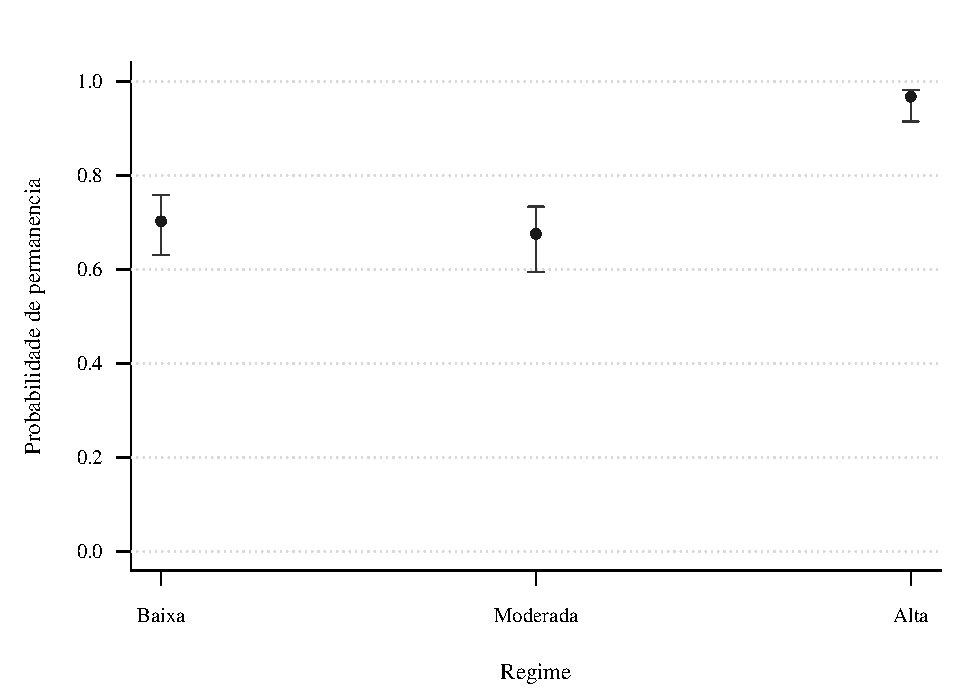
\includegraphics[width=0.75\textwidth]{resultados_markov_ipca/grafico_05_ic_persistencia_bootstrap.pdf}
\caption{Persistencia dos regimes com estimativa MLE e intervalos de confianca bootstrap suavizado.}
\label{fig:bootstrap_persistencia}
\end{figure}

Mesmo apos considerar a incerteza amostral, a persistencia do regime de alta inflacao permanece elevada. O intervalo bootstrap para \(p_{AA}\) vai de 0,9146 a 0,9820, reforcando a conclusao de que episodios de alta inflacao tendem a ser persistentes na amostra completa.

Foram realizados tres testes LR. O primeiro compara a cadeia de Markov com um modelo de independencia temporal. A hipotese nula e que o regime em \(t+1\) independe do regime em \(t\). O segundo teste compara a especificacao de primeira ordem com uma cadeia de segunda ordem. O terceiro teste avalia a estabilidade temporal das matrizes. Alem dos p-valores assintoticos, foram calculados p-valores por Monte Carlo com \(B=1000\) simulacoes e correcao
\[
\widehat{p}_{MC}=\frac{1+\#\{LR_b\geq LR_{\text{obs}}\}}{B+1}.
\]
No teste de independencia temporal, as sequencias simuladas foram geradas sob a hipotese nula iid, usando as frequencias marginais dos regimes. No teste de primeira contra segunda ordem, as sequencias foram simuladas a partir da cadeia de primeira ordem estimada com suavizacao \(\alpha=0,5\). Nos testes de estabilidade, as sequencias foram simuladas sob a matriz comum estimada pela agregacao das contagens dos grupos comparados, tambem suavizada com \(\alpha=0,5\), preservando o tamanho de cada subamostra.

O resultado rejeita fortemente a independencia temporal, tanto pela aproximacao qui-quadrado quanto por Monte Carlo. Para a comparacao entre primeira e segunda ordem, o p-valor assintotico e 0,2596, mas o p-valor por Monte Carlo e 0,0470. Essa divergencia recomenda cautela, pois alguns contextos de segunda ordem sao raros ou nao observados. Assim, a cadeia de primeira ordem e mantida como especificacao principal por parcimonia e interpretabilidade, mas nao deve ser tratada como verdade definitiva.

\begin{table}[H]
\centering
\caption{Testes LR e p-valores por Monte Carlo}
\label{tab:testes_lr}
\begin{tabular}{lccc}
\hline
Teste & Estatistica LR & p-valor assintotico & p-valor Monte Carlo \\
\hline
Dependencia temporal vs. independencia & 673,78 & \(1,65\times 10^{-144}\) & 0,0010 \\
Primeira ordem vs. segunda ordem & 14,68 & 0,2596 & 0,0470 \\
Estabilidade pre-Real vs. pos-Real & 27,53 & 0,0001 & 0,0010 \\
Estabilidade pre-pandemia/pandemia/pos-pandemia & 13,44 & 0,3379 & 0,1409 \\
\hline
\end{tabular}
\end{table}

A evidencia mais forte e a rejeicao da independencia temporal e da estabilidade pre-Real versus pos-Real. A comparacao entre pre-pandemia, pandemia e pos-pandemia nao rejeita estabilidade aos niveis usuais, sugerindo que a ruptura historica central na amostra e a associada ao Plano Real.

\subsection{Mudanca historica: pre-Real e pos-Real}

A amostra completa mistura dois regimes macroeconomicos distintos. Antes de julho de 1994, a economia brasileira conviveu com inflacao cronica e episodios de inflacao mensal muito elevada. Depois do Plano Real, a dinamica inflacionaria passou a ocorrer em escala muito inferior. Por isso, a analise principal do trabalho deve ser a comparacao entre pre-Real e pos-Real.

Para a analise descritiva por subperiodo, os tercis foram recalculados dentro de cada amostra. Essa decisao torna os estados relativos ao ambiente historico analisado. Portanto, ``Alta'' no pre-Real significa o terco superior da inflacao dentro de uma economia de inflacao cronica; ``Alta'' no pos-Real significa o terco superior dentro de uma economia estabilizada. As categorias nao representam os mesmos niveis absolutos de inflacao.

\begin{table}[H]
\centering
\caption{Limiares por subperiodo com tercis proprios}
\label{tab:limiares_pre_pos}
\begin{tabular}{llc}
\hline
Periodo & Limite & IPCA mensal (\%) \\
\hline
Pre-Real & Baixa--Moderada & 8,44 \\
Pre-Real & Moderada--Alta & 18,59 \\
Pos-Real & Baixa--Moderada & 0,33 \\
Pos-Real & Moderada--Alta & 0,60 \\
\hline
\end{tabular}
\end{table}

A diferenca entre os limiares e substantiva. No pre-Real, o limite entre inflacao moderada e alta e 18,59\% ao mes. No pos-Real, o limite equivalente e 0,60\% ao mes. Isso confirma que a comparacao entre subperiodos precisa ser feita com cuidado: a analise por tercis proprios compara persistencia relativa dentro de cada ambiente, nao niveis absolutos de inflacao.

\begin{table}[H]
\centering
\caption{Persistencia por subperiodo com tercis proprios}
\label{tab:persistencia_pre_pos}
\begin{tabular}{llcc}
\hline
Periodo & Regime & Probabilidade de permanencia & Duracao esperada (meses) \\
\hline
Pre-Real & Baixa    & 0,8276 & 5,80 \\
Pre-Real & Moderada & 0,7241 & 3,63 \\
Pre-Real & Alta     & 0,8947 & 9,50 \\
Pos-Real & Baixa    & 0,6066 & 2,54 \\
Pos-Real & Moderada & 0,4737 & 1,90 \\
Pos-Real & Alta     & 0,6508 & 2,86 \\
\hline
\end{tabular}
\end{table}

\begin{figure}[H]
\centering
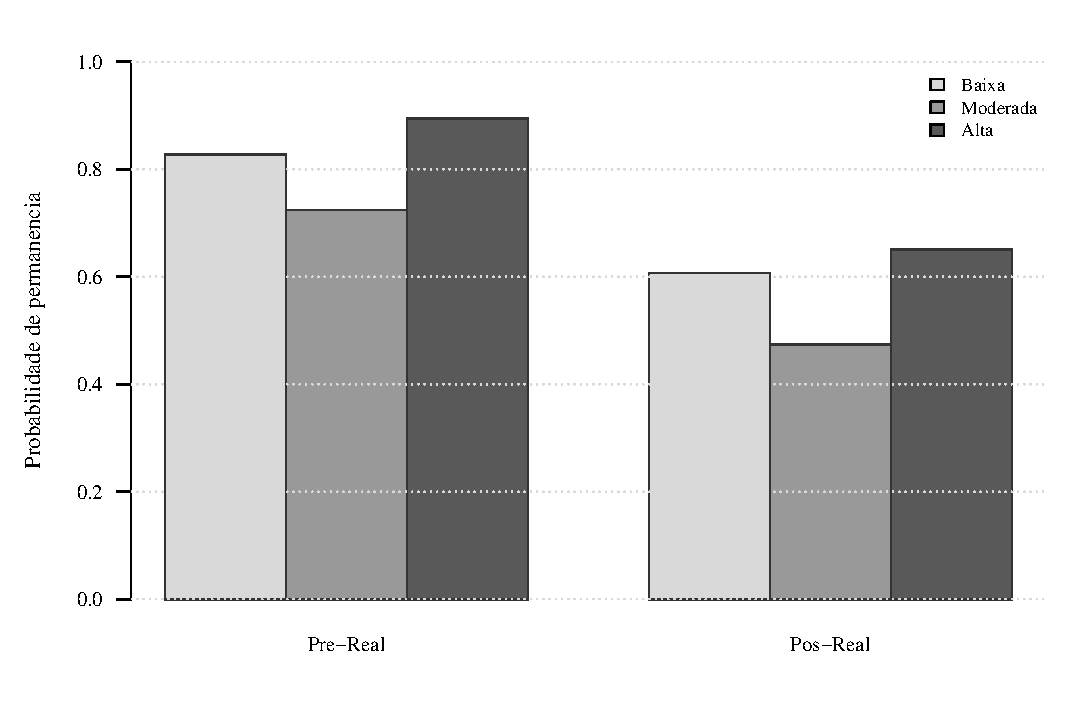
\includegraphics[width=0.78\textwidth]{resultados_markov_ipca/grafico_10_persistencia_pre_pos_real.pdf}
\caption{Persistencia dos regimes nos periodos pre-Real e pos-Real.}
\label{fig:persistencia_pre_pos}
\end{figure}

\begin{figure}[H]
\centering
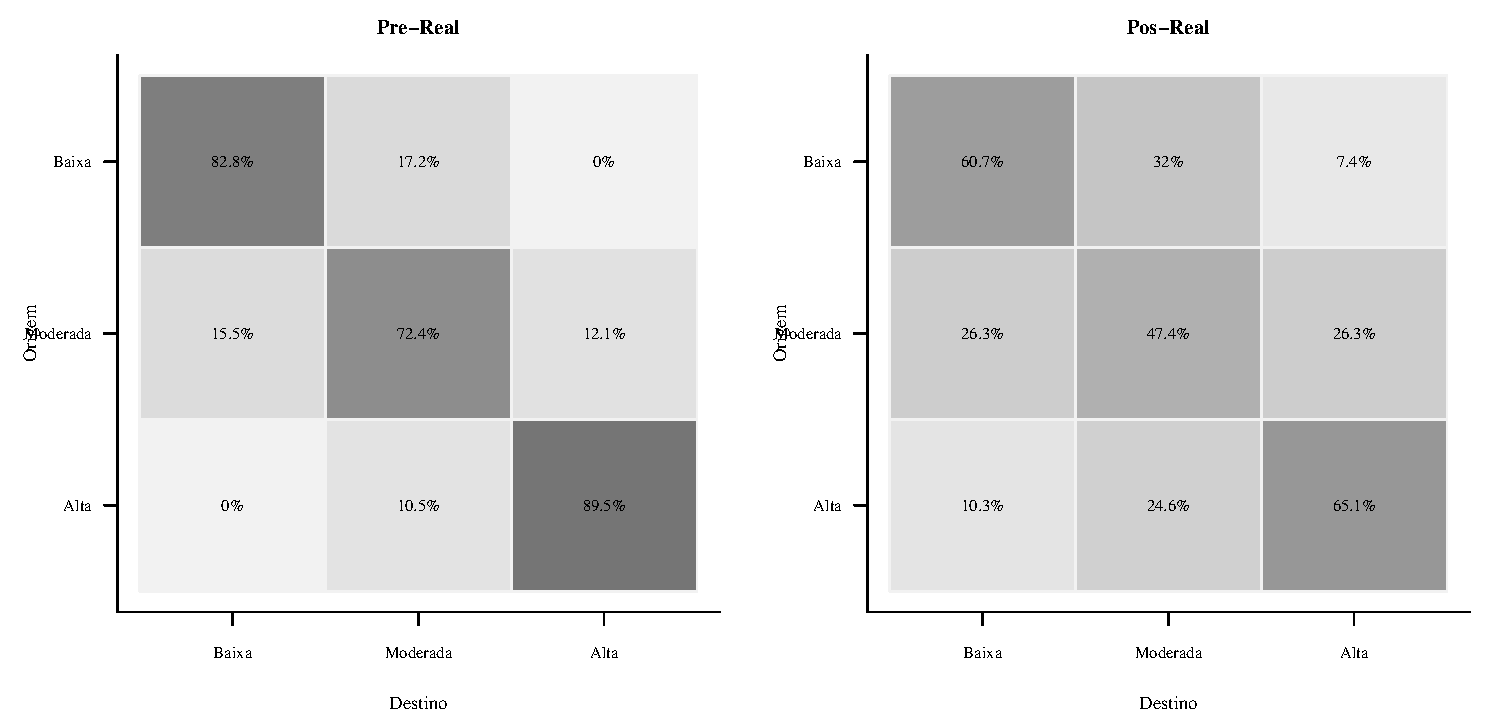
\includegraphics[width=0.95\textwidth]{resultados_markov_ipca/grafico_11_matrizes_pre_pos_real.pdf}
\caption{Matrizes de transicao estimadas separadamente para os periodos pre-Real e pos-Real.}
\label{fig:matrizes_pre_pos}
\end{figure}

A Tabela \ref{tab:persistencia_pre_pos} e as Figuras \ref{fig:persistencia_pre_pos} e \ref{fig:matrizes_pre_pos} mostram queda expressiva da persistencia apos a estabilizacao. No pre-Real, o regime de alta inflacao tinha probabilidade de permanencia de 0,8947 e duracao esperada de 9,50 meses. No pos-Real, a permanencia no regime alto cai para 0,6508 e a duracao esperada para 2,86 meses. A matriz pos-Real tambem mostra maior frequencia de transicoes entre regimes, inclusive transicoes diretas entre estados extremos, que nao apareciam na matriz agregada.

O teste formal pre-Real versus pos-Real usa os regimes globais da amostra completa, e nao os tercis recalculados dentro de cada subperiodo, porque a igualdade de matrizes exige que os estados tenham a mesma definicao. O teste rejeita estabilidade: \(LR=27,53\), com p-valor assintotico de 0,0001 e p-valor Monte Carlo de 0,0010. Portanto, ha evidencia estatistica de que a matriz de transicao mudou apos o Plano Real.

\subsection{Extensoes exploratorias e robustez auxiliar}

As analises anteriores constituem o nucleo empirico do trabalho. Como exercicios auxiliares, foram estimadas tres extensoes: agrupamento por \(k\)-means, HMM gaussiano e um modelo aproximado de probabilidades de transicao variaveis no tempo. Essas extensoes nao devem ser lidas como robustez forte no sentido de validacao independente completa. Elas funcionam como diagnosticos exploratorios de sensibilidade a escala, classificacao latente e covariaveis macroeconomicas.

O \(k\)-means em nivel foi fortemente influenciado pelos valores extremos do periodo pre-Real, com centros estimados de 1,50\%, 18,39\% e 45,35\% ao mes. Por isso, foi estimada tambem uma versao em \(\log(1+\text{IPCA})\). Nessa transformacao, os centros aproximados na escala original foram 0,49\%, 7,41\% e 25,47\%. O resultado confirma que metodos baseados diretamente na escala do IPCA sao sensiveis a outliers historicos.

O HMM gaussiano trata os regimes como estados latentes nao observados. O modelo foi estimado por EM com filtro forward-backward escalado, inicializacao por \(k\)-means com \(nstart=100\), tolerancia \(10^{-8}\) e ordenacao dos estados pelas medias estimadas. Em nivel, o HMM apresentou log-verossimilhanca \(-843,44\), AIC 1714,88, BIC 1775,37 e convergiu em 33 iteracoes. Em \(\log(1+\text{IPCA})\), apresentou log-verossimilhanca \(-189,74\), AIC 407,47, BIC 467,96 e convergiu em 21 iteracoes. O modelo em \(\log(1+\text{IPCA})\) estimou medias aproximadas de 0,51\%, 7,96\% e 25,88\% para os tres regimes latentes. As probabilidades suavizadas mostram que o modelo capta principalmente a separacao entre inflacao cronica e estabilizacao. Por isso, o HMM deve permanecer como apendice exploratorio, e nao como evidencia central do trabalho. Uma robustez forte exigiria comparar inicializacoes alternativas, estabilidade dos estados latentes e desempenho preditivo fora da amostra.

Por fim, foi estimado um modelo aproximado de probabilidades de transicao variaveis no tempo. A especificacao foi restrita ao periodo pos-Real e usou os tercis proprios desse subperiodo, pois a Selic Meta e economicamente mais coerente no ambiente de estabilizacao. O modelo estimado foi um logit multinomial com interacoes entre o regime de origem e as covariaveis:
\[
\Pr(X_{t+1}=j\mid X_t=i,Z_t)
=
\frac{\exp(\alpha_{ij}+\beta_{ij}'Z_t)}
{\sum_{\ell}\exp(\alpha_{i\ell}+\beta_{i\ell}'Z_t)},
\]
em que \(Z_t\) inclui o IPCA mensal de origem e a Selic Meta de origem, ambos padronizados. O modelo nulo usado no teste LR contem apenas o regime de origem. A amostra efetiva do TVTP e de 324 transicoes, de abril de 1999 a marco de 2026.

\begin{table}[H]
\centering
\caption{Coeficientes do logit multinomial TVTP no periodo pos-Real}
\label{tab:tvtp_coeficientes}
\scriptsize
\begin{tabular}{llrrr}
\hline
Destino & Variavel & Coeficiente & Erro-padrao & p-valor \\
\hline
Moderada & Intercepto & 0,7147 & 0,6728 & 0,2881 \\
Moderada & Origem = Moderada & 0,7065 & 0,7981 & 0,3760 \\
Moderada & Origem = Alta & 0,0281 & 0,8581 & 0,9739 \\
Moderada & IPCA\(_t\) & 1,8051 & 0,9241 & 0,0508 \\
Moderada & Selic\(_t\) & 0,0317 & 0,2181 & 0,8843 \\
Moderada & Origem Moderada \(\times\) IPCA\(_t\) & 1,9723 & 1,9457 & 0,3107 \\
Moderada & Origem Alta \(\times\) IPCA\(_t\) & -1,9429 & 1,2867 & 0,1310 \\
Moderada & Origem Moderada \(\times\) Selic\(_t\) & -0,0125 & 0,3443 & 0,9710 \\
Moderada & Origem Alta \(\times\) Selic\(_t\) & -0,2454 & 0,3970 & 0,5365 \\
Alta & Intercepto & 1,9155 & 1,8298 & 0,2952 \\
Alta & Origem = Moderada & -1,1417 & 1,8901 & 0,5458 \\
Alta & Origem = Alta & -0,9848 & 1,8918 & 0,6027 \\
Alta & IPCA\(_t\) & 6,0494 & 3,1265 & 0,0530 \\
Alta & Selic\(_t\) & -0,0137 & 0,3610 & 0,9698 \\
Alta & Origem Moderada \(\times\) IPCA\(_t\) & -1,9834 & 3,6938 & 0,5913 \\
Alta & Origem Alta \(\times\) IPCA\(_t\) & -5,0142 & 3,2145 & 0,1188 \\
Alta & Origem Moderada \(\times\) Selic\(_t\) & 0,1081 & 0,4670 & 0,8170 \\
Alta & Origem Alta \(\times\) Selic\(_t\) & -0,1543 & 0,4682 & 0,7417 \\
\hline
\end{tabular}
\begin{flushleft}
\footnotesize Nota: a categoria de destino de referencia e Baixa. IPCA\(_t\) e Selic\(_t\) foram padronizados. Os coeficientes indicam associacao estatistica no logit multinomial; nao possuem interpretacao causal.
\end{flushleft}
\end{table}

\begin{table}[H]
\centering
\caption{Diagnostico do ajuste do modelo TVTP}
\label{tab:tvtp_diagnostico}
\begin{tabular}{lc}
\hline
Indicador & Valor \\
\hline
Amostra efetiva & 324 \\
Numero de parametros & 18 \\
Log-verossimilhanca & -298,02 \\
AIC & 632,04 \\
BIC & 700,10 \\
Codigo de convergencia & 0 \\
Convergiu & Sim \\
Menor contagem em celula origem-destino & 9 \\
Celulas origem-destino com zero & 0 \\
Maior \(|\widehat{\beta}|\) & 6,0494 \\
Menor probabilidade prevista & \(1,61\times 10^{-5}\) \\
Alerta de quase-separacao & Nao \\
\hline
\end{tabular}
\end{table}

O diagnostico de quase-separacao adotou o seguinte criterio operacional: alerta se o maior coeficiente absoluto fosse superior a 10, se a menor probabilidade prevista fosse inferior a \(10^{-6}\), ou se houvesse celula origem-destino com contagem zero na amostra efetiva do TVTP. Nenhuma dessas condicoes ocorreu. Ainda assim, como alguns coeficientes sao grandes e os erros-padrao tambem sao elevados, a interpretacao deve privilegiar o teste global e as probabilidades previstas, nao coeficientes individuais isolados.

\begin{table}[H]
\centering
\caption{Probabilidades medias previstas pelo modelo TVTP no periodo pos-Real}
\label{tab:tvtp_probabilidades}
\begin{tabular}{lccc}
\hline
Origem & Baixa & Moderada & Alta \\
\hline
Baixa    & 0,5888 & 0,3271 & 0,0841 \\
Moderada & 0,2562 & 0,4959 & 0,2479 \\
Alta     & 0,1354 & 0,2604 & 0,6042 \\
\hline
\end{tabular}
\end{table}

O teste LR do TVTP contra o modelo com origem apenas resultou em \(LR=23,47\), com 12 graus de liberdade e p-valor 0,0240. Esse resultado sugere que as covariaveis macroeconomicas ajudam a explicar as probabilidades de transicao no periodo pos-Real. A Tabela \ref{tab:tvtp_probabilidades}, contudo, nao deve ser interpretada como uma matriz de transicao fixa. Ela apresenta medias das probabilidades previstas, que variam mes a mes conforme o IPCA e a Selic observados. Tambem nao se deve interpretar o modelo como evidencia causal de politica monetaria, pois a Selic reage ao ambiente inflacionario e seus efeitos podem operar com defasagens.

\begin{figure}[H]
\centering
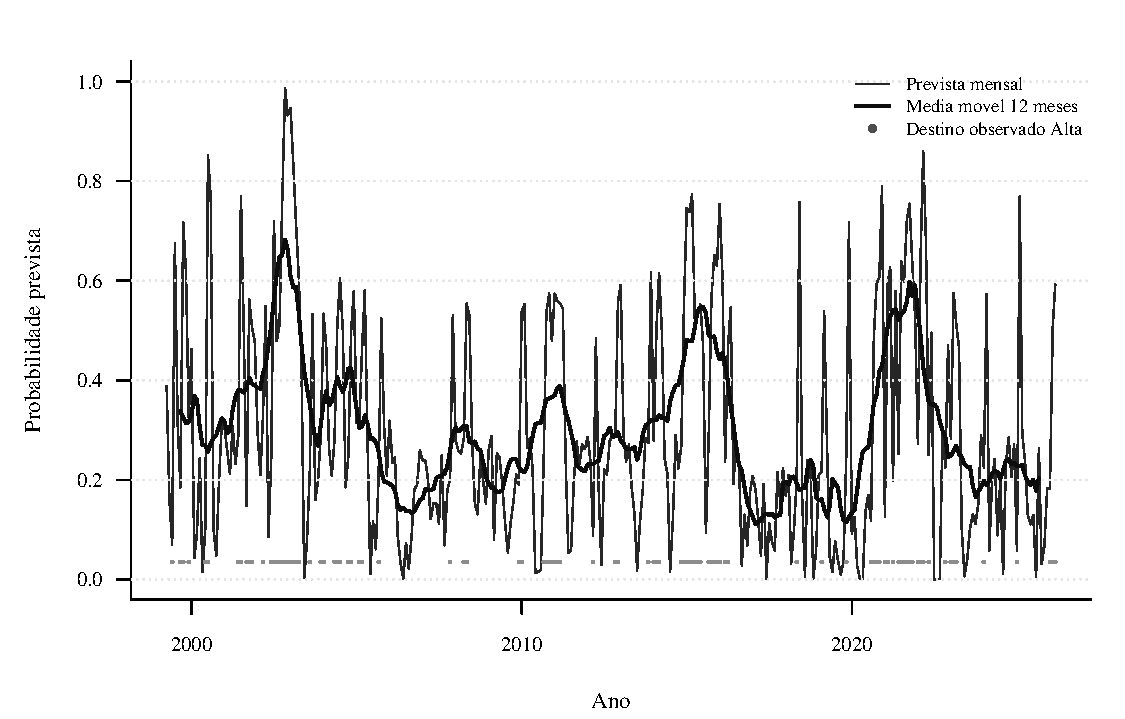
\includegraphics[width=0.82\textwidth]{resultados_markov_ipca/grafico_08_tvtp_probabilidade_alta.pdf}
\caption{Probabilidade prevista de destino em regime de alta inflacao no modelo TVTP pos-Real.}
\label{fig:tvtp_alta}
\end{figure}

\subsection{Discussao e limitacoes}

Os resultados indicam que a inflacao brasileira apresenta dependencia temporal entre regimes. A rejeicao da independencia temporal mostra que a classificacao do mes anterior contem informacao relevante sobre o regime do mes seguinte. A matriz de transicao, portanto, resume uma forma substantiva de persistencia inflacionaria.

O principal resultado economico, entretanto, nao e a matriz agregada da amostra completa, mas a comparacao entre pre-Real e pos-Real. A estabilizacao monetaria reduziu a persistencia dos regimes, especialmente do regime de alta inflacao. Antes do Plano Real, a alta inflacao era muito persistente mesmo quando definida relativamente ao proprio periodo. Depois do Plano Real, a alta inflacao continua sendo o regime mais persistente do pos-Real, mas sua duracao esperada cai para menos de tres meses.

A analise possui limitacoes. Primeiro, os regimes por tercis sao categorias relativas, nao limites normativos de politica economica. Segundo, a cadeia principal e homogenea no tempo dentro da amostra considerada, embora a evidencia mostre quebra estrutural relevante. Terceiro, os testes LR assintoticos podem ser sensiveis a zeros e celulas raras; por isso foram reportados p-valores de Monte Carlo. Quarto, as extensoes por \(k\)-means, HMM e TVTP sao verificacoes auxiliares, nao substitutos do resultado principal. Quinto, nem todos os conceitos do referencial teorico sao operacionalizados empiricamente: tempo continuo, acoplamento e dependencia fraca aparecem como extensoes conceituais, enquanto a aplicacao efetiva se concentra em cadeias finitas de tempo discreto, inferencia por transicoes observadas e diagnosticos espectrais da matriz estimada. Por fim, o trabalho nao realiza validacao preditiva fora da amostra; as conclusoes devem ser entendidas como descricao estatistica da dinamica historica do IPCA.

\subsection{Conclusao da aplicacao}

A aplicacao ao IPCA mostra que cadeias de Markov oferecem uma ferramenta simples, interpretavel e estatisticamente rica para estudar regimes inflacionarios. A matriz de transicao da amostra completa revela elevada persistencia da alta inflacao, mas essa leitura agregada precisa ser relativizada pela mudanca estrutural do Plano Real. Quando a amostra e separada em pre-Real e pos-Real, observa-se queda expressiva na duracao esperada dos regimes, sobretudo da alta inflacao. Assim, a principal conclusao empirica e que a dinamica inflacionaria brasileira apresenta dependencia temporal, mas essa dependencia nao e historicamente estavel: ela muda de forma substantiva apos a estabilizacao monetaria.
